\documentclass[11pt]{article}
\usepackage{fullpage}
\usepackage{graphics,epsfig,color}
\usepackage{wrapfig}
\usepackage{amsmath}
\usepackage{forest}
\usepackage{times}
\usepackage{setspace}
\usepackage{amsmath,amsthm,amssymb}
\usepackage{subfigure}
\usepackage{url}
\newtheorem{problem}{Problem}
\newtheorem{answer}{Answer}
\usepackage{listings}
\usepackage{color}
\usepackage{adjustbox}
\usepackage{tikz}

\definecolor{dkgreen}{rgb}{0,0.6,0}
\definecolor{gray}{rgb}{0.5,0.5,0.5}
\definecolor{mauve}{rgb}{0.58,0,0.82}

\lstset{frame=tb,
	language=Java,
	aboveskip=3mm,
	belowskip=3mm,
	showstringspaces=false,
	columns=flexible,
	basicstyle={\small\ttfamily},
	numbers=none,
	numberstyle=\tiny\color{gray},
	keywordstyle=\color{blue},
	commentstyle=\color{dkgreen},
	stringstyle=\color{mauve},
	breaklines=true,
	breakatwhitespace=true,
	tabsize=3
}

\usetikzlibrary{arrows,trees,positioning}

\tikzset{
	treenode/.style = {align=center, inner sep=0pt, text centered,
		font=\sffamily},
	arn_n/.style = {treenode, circle, white, font=\sffamily\bfseries, draw=black,
		fill=black, text width=1.5em},% arbre rouge noir, noeud noir
	arn_r/.style = {treenode, circle, red, draw=red, 
		text width=1.5em, very thick},% arbre rouge noir, noeud rouge
	arn_x/.style = {treenode, rectangle, draw=black,
		minimum width=0.5em, minimum height=0.5em}% arbre rouge noir, nil
}

\begin{document}
\begin{center}
	{\LARGE CSCD320 Homework4}
	
	\bigskip
	
	{\Large Ethan Tuning}
\end{center}

\bigskip

\begin{problem}
\label{prob:1}
 Show the trace of the construction the Red-Black tree for the sequence 12, 19, 17, 21, 16, 15. That is, you need to draw the state of the tree after inserting each number.
\end{problem}

\begin{answer}
\label{ans:1} The following pictures show the R-B tree after the keys have been added from left to right from the problem.

\bigskip
\bigskip

\begin{center}

\begin{tikzpicture}[->,>=stealth',level/.style={sibling distance = 3cm/#1,
	level distance = 1.5cm}] 
\node [arn_n] {12};
\end{tikzpicture}

\bigskip
\bigskip

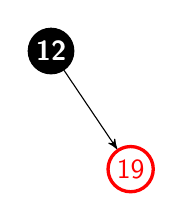
\begin{tikzpicture}[->,>=stealth',level/.style={sibling distance = 3cm/#1,
	level distance = 1.5cm}] 
\node [arn_n] {12}
	child{ node [arn_r, right = 2em] {19}}; 
\end{tikzpicture}

\bigskip
\bigskip

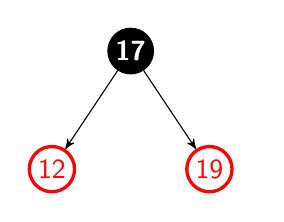
\begin{tikzpicture}[->,>=stealth',level/.style={sibling distance = 2cm/#1,
	level distance = 1.5cm}] 
\node [arn_n] {17}
child{ node [arn_r] {12}}
child{ node [arn_r,] {19} node[above right= 2em and -2em] {} node[right = 1em]{}}; 
\end{tikzpicture}

\bigskip
\bigskip

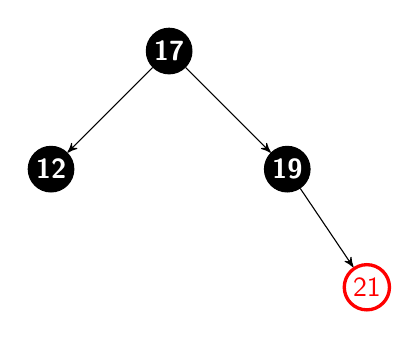
\begin{tikzpicture}[->,>=stealth',level/.style={sibling distance = 3cm/#1,
	level distance = 1.5cm}] 
\node [arn_n] {17}
child{ node [arn_n] {12}}
child{ node [arn_n] {19}
	child{node[arn_r, right = 2em] {21} node[above right= 2em and -2em] {} node[right = 1em]{} }	
};  
\end{tikzpicture}

\bigskip
\bigskip

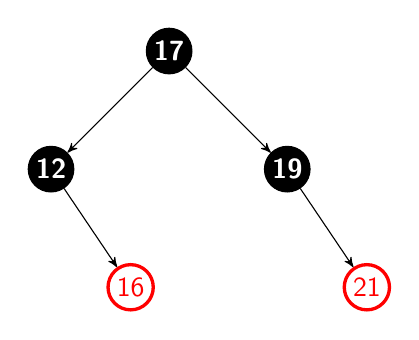
\begin{tikzpicture}[->,>=stealth',level/.style={sibling distance = 3cm/#1,
	level distance = 1.5cm}] 
\node [arn_n] {17}
child{ node [arn_n] {12}
	child{ node [arn_r, right = 2em] {16}}
}
child{ node [arn_n,] {19}
	child{node[arn_r, right = 2em] {21} node[above right= 2em and -2em] {} node[right = 1em]{} }	
};  
\end{tikzpicture}

\bigskip
\bigskip

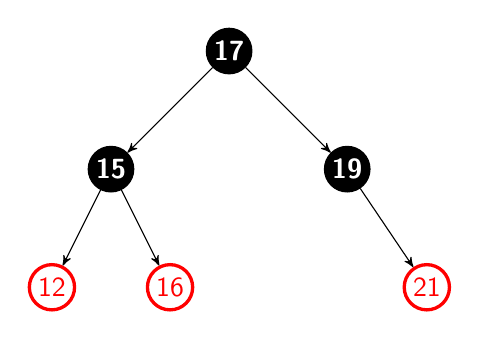
\begin{tikzpicture}[->,>=stealth',level/.style={sibling distance = 3cm/#1,
	level distance = 1.5cm}] 
\node [arn_n] {17}
child{ node [arn_n] {15}
	child{ node [arn_r] {12}}
	child{ node [arn_r] {16}}
}
child{ node [arn_n,] {19}
	child{node[arn_r, right = 2em] {21} node[above right= 2em and -2em] {} node[right = 1em]{} }	
};  
\end{tikzpicture}
\end{center}
\end{answer}

\bigskip

\begin{problem}
\label{prob:2}
 Show the trace of deleting the nodes from the Red-Black tree below in the order of 14, 1, 5, 2, 11, 7, 15, 8. That is, show the state of the tree after deleting each node.

\bigskip
\bigskip
\begin{center}
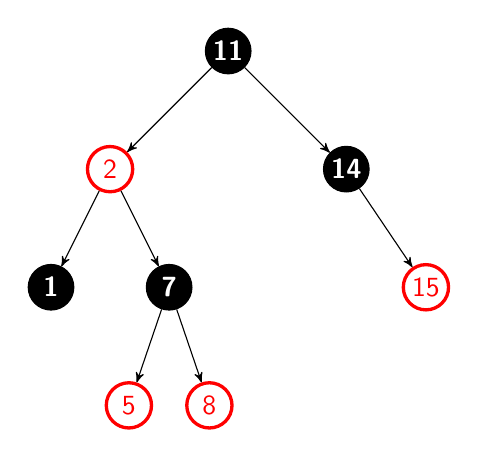
\begin{tikzpicture}[->,>=stealth',level/.style={sibling distance = 3cm/#1,
	level distance = 1.5cm}] 
\node [arn_n] {11}
child{ node [arn_r] {2}
	child{ node [arn_n] {1}}
	child{ node [arn_n] {7}
		child{ node [arn_r, right = 2em] {8}}
		child{ node [arn_r, left = 2em] {5}}
	}
}
child{ node [arn_n,] {14}
	child{node[arn_r, right = 2em] {15} node[above right= 2em and -2em] {} node[right = 1em]{} }	
}; 
\end{tikzpicture}
\end{center}
\end{problem}

\bigskip

\begin{answer}
\label{ans:2} The following pictures show the R-B tree after the keys have been deleted from left to right from the problem.

\bigskip
\bigskip

\begin{center}
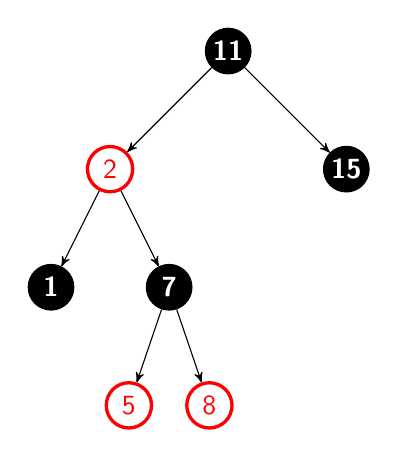
\begin{tikzpicture}[->,>=stealth',level/.style={sibling distance = 3cm/#1,
	level distance = 1.5cm}] 
\node [arn_n] {11}
child{ node [arn_r] {2}
	child{ node [arn_n] {1}}
	child{ node [arn_n] {7}
		child{ node [arn_r, right = 2em] {8}}
		child{ node [arn_r, left = 2em] {5}}
	}
}
child{ node [arn_n,] {15}}; 
\end{tikzpicture}

\bigskip
\bigskip

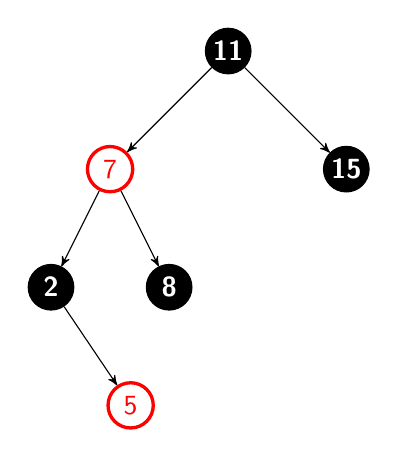
\begin{tikzpicture}[->,>=stealth',level/.style={sibling distance = 3cm/#1,
	level distance = 1.5cm}] 
\node [arn_n] {11}
	child{ node [arn_r] {7}
		child{ node[arn_n] {2}
			child{ node[arn_r, right = 2em] {5}}
		}
		child{ node[arn_n] {8}
		}
	}
child{ node [arn_n,] {15}}; 
\end{tikzpicture}

\bigskip
\bigskip

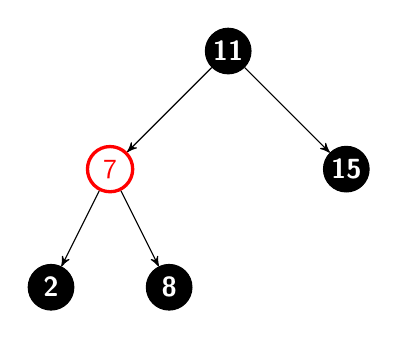
\begin{tikzpicture}[->,>=stealth',level/.style={sibling distance = 3cm/#1,
	level distance = 1.5cm}] 
\node [arn_n] {11}
child{ node [arn_r] {7}
	child{ node[arn_n] {2}}
	child{ node[arn_n] {8}}
}
child{ node [arn_n,] {15}}; 
\end{tikzpicture}

\bigskip
\bigskip

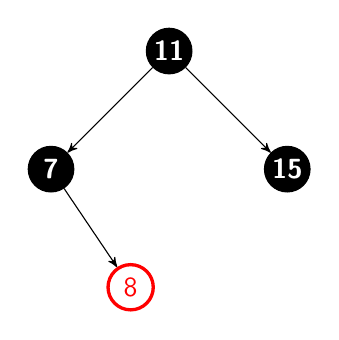
\begin{tikzpicture}[->,>=stealth',level/.style={sibling distance = 3cm/#1,
	level distance = 1.5cm}] 
\node [arn_n] {11}
child{ node [arn_n] {7}
	child{ node[arn_r, right = 2em] {8}}
}
child{ node [arn_n,] {15}}; 
\end{tikzpicture}

\bigskip
\bigskip

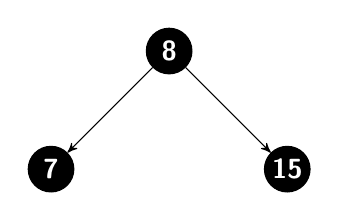
\begin{tikzpicture}[->,>=stealth',level/.style={sibling distance = 3cm/#1,
	level distance = 1.5cm}] 
\node [arn_n] {8}
child{ node [arn_n] {7}}
child{ node [arn_n,] {15}}; 
\end{tikzpicture}

\bigskip
\bigskip

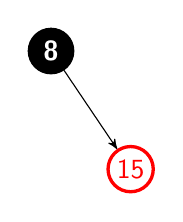
\begin{tikzpicture}[->,>=stealth',level/.style={sibling distance = 3cm/#1,
	level distance = 1.5cm}] 
\node [arn_n] {8}
child{ node [arn_r, right = 2em] {15}}; 
\end{tikzpicture}

\bigskip
\bigskip


\begin{tikzpicture}[->,>=stealth',level/.style={sibling distance = 3cm/#1,
	level distance = 1.5cm}] 
\node [arn_n] {8};
\end{tikzpicture}
\end{center}
\end{answer}

\bigskip

\begin{problem}
\label{prob:3}
 Trace the ONE-PASS construction of the B-tree for the sequence ${M,C,P,H,G,X,S,U,O,A,W}$. Draw the configuration of the B-tree after inserting each letter. We use t = 2 as the branching degree threshold of the B-tree, so that: $(1)$ all the non-leaf nodes must have at least $t - 1 = 1$ keys and at most $2t - 1 = 3$ keys; and $(2)$ The root node of an non-empty B-tree must have at least one key and at most $2t - 1 = 3$ keys.
\end{problem}

\begin{answer}
\label{ans:3} The following pictures show the B-tree after the keys have been added from left to right from the problem.
\begin{center}

\begin{tikzpicture}
\tikzstyle{bplus}=[rectangle split, rectangle split horizontal,rectangle split ignore empty parts,draw]
\tikzstyle{every node}=[bplus]
\tikzstyle{level 1}=[sibling distance=60mm]
\tikzstyle{level 2}=[sibling distance=15mm]
\node {M};
\end{tikzpicture}

\bigskip
\bigskip

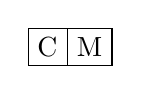
\begin{tikzpicture}
\tikzstyle{bplus}=[rectangle split, rectangle split horizontal,rectangle split ignore empty parts,draw]
\tikzstyle{every node}=[bplus]
\tikzstyle{level 1}=[sibling distance=60mm]
\tikzstyle{level 2}=[sibling distance=15mm]
\node {C \nodepart{two} M};
\end{tikzpicture}

\bigskip
\bigskip

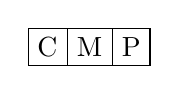
\begin{tikzpicture}
\tikzstyle{bplus}=[rectangle split, rectangle split horizontal,rectangle split ignore empty parts,draw]
\tikzstyle{every node}=[bplus]
\tikzstyle{level 1}=[sibling distance=30mm]
\tikzstyle{level 2}=[sibling distance=15mm]
\node {C \nodepart{two} M \nodepart{three} P};
\end{tikzpicture}

\bigskip
\bigskip

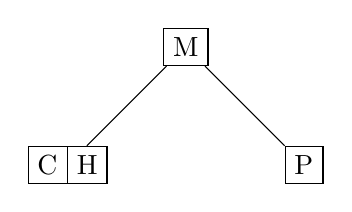
\begin{tikzpicture}
\tikzstyle{bplus}=[rectangle split, rectangle split horizontal,rectangle split ignore empty parts,draw]
\tikzstyle{every node}=[bplus]
\tikzstyle{level 1}=[sibling distance=30mm]
\tikzstyle{level 2}=[sibling distance=15mm]
\node {M}
child {node {C \nodepart{two} H}}
child {node {P}};
\end{tikzpicture}

\bigskip
\bigskip

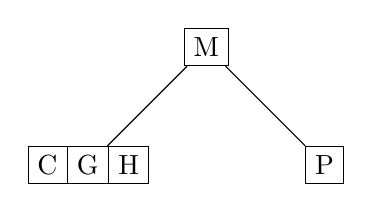
\begin{tikzpicture}
\tikzstyle{bplus}=[rectangle split, rectangle split horizontal,rectangle split ignore empty parts,draw]
\tikzstyle{every node}=[bplus]
\tikzstyle{level 1}=[sibling distance=30mm]
\tikzstyle{level 2}=[sibling distance=15mm]
\node {M}
child {node {C \nodepart{two} G \nodepart{three} H}}
child {node {P}};
\end{tikzpicture}

\bigskip
\bigskip

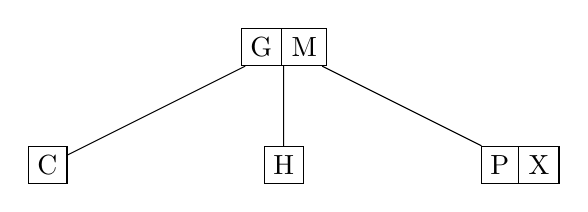
\begin{tikzpicture}
\tikzstyle{bplus}=[rectangle split, rectangle split horizontal,rectangle split ignore empty parts,draw]
\tikzstyle{every node}=[bplus]
\tikzstyle{level 1}=[sibling distance=30mm]
\tikzstyle{level 2}=[sibling distance=15mm]
\node {G \nodepart{two} M}
child {node {C}}
child {node {H}}
child {node {P \nodepart{two} X}};
\end{tikzpicture}

\bigskip
\bigskip

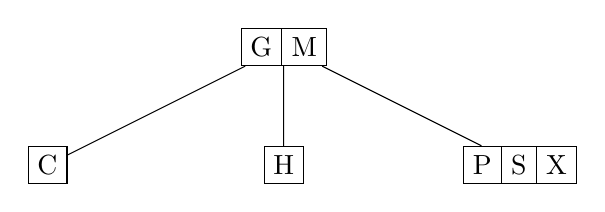
\begin{tikzpicture}
\tikzstyle{bplus}=[rectangle split, rectangle split horizontal,rectangle split ignore empty parts,draw]
\tikzstyle{every node}=[bplus]
\tikzstyle{level 1}=[sibling distance=30mm]
\tikzstyle{level 2}=[sibling distance=15mm]
\node {G \nodepart{two} M}
child {node {C}}
child {node {H}}
child {node {P \nodepart{two} S \nodepart{three} X}};
\end{tikzpicture}

\bigskip
\bigskip

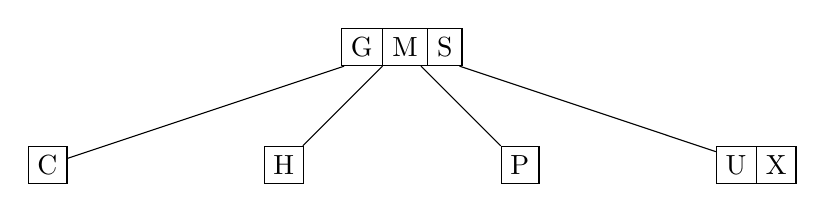
\begin{tikzpicture}
\tikzstyle{bplus}=[rectangle split, rectangle split horizontal,rectangle split ignore empty parts,draw]
\tikzstyle{every node}=[bplus]
\tikzstyle{level 1}=[sibling distance=30mm]
\tikzstyle{level 2}=[sibling distance=15mm]
\node {G \nodepart{two} M \nodepart{three} S}
child {node {C}}
child {node {H}}
child {node {P}}
child {node {U \nodepart{two} X}};
\end{tikzpicture}

\bigskip
\bigskip

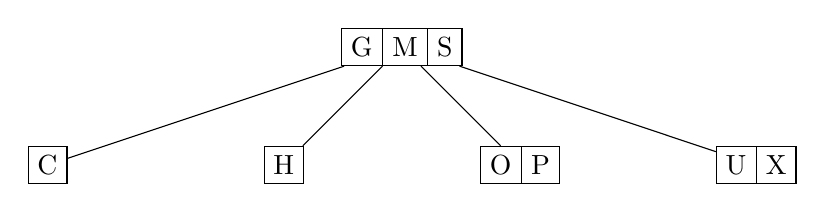
\begin{tikzpicture}
\tikzstyle{bplus}=[rectangle split, rectangle split horizontal,rectangle split ignore empty parts,draw]
\tikzstyle{every node}=[bplus]
\tikzstyle{level 1}=[sibling distance=30mm]
\tikzstyle{level 2}=[sibling distance=15mm]
\node {G \nodepart{two} M \nodepart{three} S}
child {node {C}}
child {node {H}}
child {node {O \nodepart{three} P}}
child {node {U \nodepart{two} X}};
\end{tikzpicture}

\bigskip
\bigskip

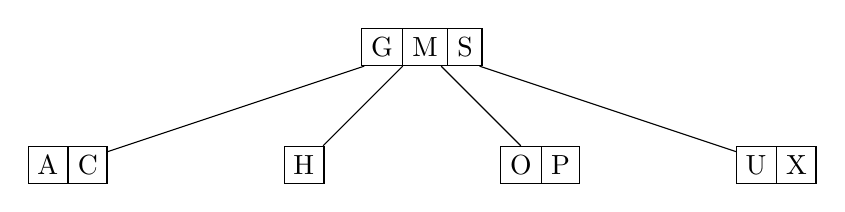
\begin{tikzpicture}
\tikzstyle{bplus}=[rectangle split, rectangle split horizontal,rectangle split ignore empty parts,draw]
\tikzstyle{every node}=[bplus]
\tikzstyle{level 1}=[sibling distance=30mm]
\tikzstyle{level 2}=[sibling distance=15mm]
\node {G \nodepart{two} M \nodepart{three} S}
child {node {A \nodepart{two} C}}
child {node {H}}
child {node {O \nodepart{three} P}}
child {node {U \nodepart{two} X}};
\end{tikzpicture}

\bigskip
\bigskip

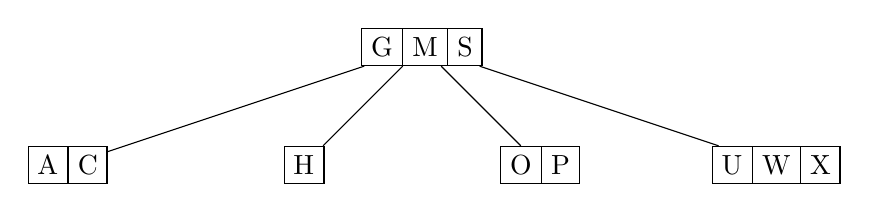
\begin{tikzpicture}
\tikzstyle{bplus}=[rectangle split, rectangle split horizontal,rectangle split ignore empty parts,draw]
\tikzstyle{every node}=[bplus]
\tikzstyle{level 1}=[sibling distance=30mm]
\tikzstyle{level 2}=[sibling distance=15mm]
\node {G \nodepart{two} M \nodepart{three} S}
child {node {A \nodepart{two} C}}
child {node {H}}
child {node {O \nodepart{three} P}}
child {node {U \nodepart{two} W \nodepart{three} X}};
\end{tikzpicture}
\end{center}
\end{answer}

\bigskip

\begin{problem}
\label{prob:4}
 Trace the deletion of the sequence of keys ${G,S,Y,T,F}$ from the B-tree below. Draw the configuration of the B-tree after each deletion. We use $t = 2$ as the branching degree threshold of the B-tree, so that: $(1)$ all the non-leaf nodes must have at least $t - 1 = 1$ keys and at most $2t - 1 = 3$ keys; and $(2)$ the root node of a non-empty B-tree must have at least one key and at most $2t - 1 = 3$ keys.

\bigskip
\begin{center}
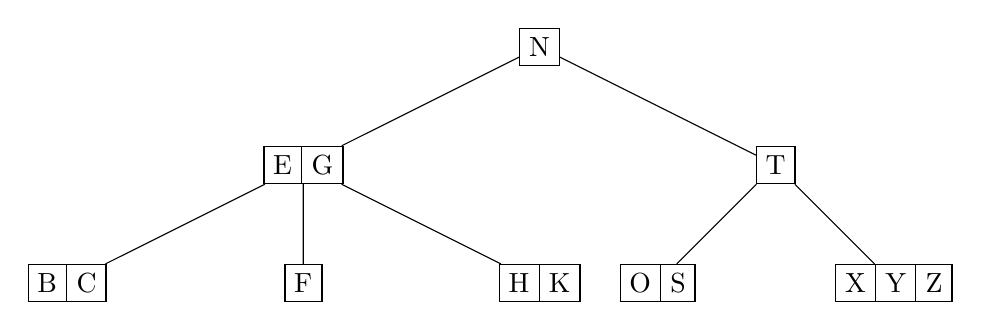
\begin{tikzpicture}
\tikzstyle{bplus}=[rectangle split, rectangle split horizontal,rectangle split ignore empty parts,draw]
\tikzstyle{every node}=[bplus]
\tikzstyle{level 1}=[sibling distance=60mm]
\tikzstyle{level 2}=[sibling distance=30mm]

\node{N}
child{ node{E \nodepart{two} G}
	child{ node{B \nodepart{two} C}}
	child{ node{F}}
	child{ node{H \nodepart{two} K}}
}
child{ node{T}
	child{ node{O \nodepart{two} S}}
	child{ node{X \nodepart{two} Y \nodepart{three} Z}}
};
\end{tikzpicture}
\end{center}
\end{problem}

\begin{answer}
\label{ans:4} The following pictures show the B-tree after the keys have been deleted from left to right from the problem.

\begin{center}
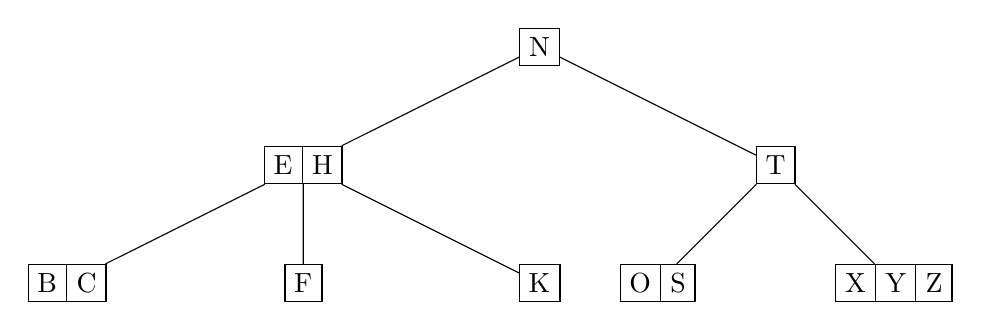
\begin{tikzpicture}
\tikzstyle{bplus}=[rectangle split, rectangle split horizontal,rectangle split ignore empty parts,draw]
\tikzstyle{every node}=[bplus]
\tikzstyle{level 1}=[sibling distance=60mm]
\tikzstyle{level 2}=[sibling distance=30mm]

\node{N}
child{ node{E \nodepart{two} H}
	child{ node{B \nodepart{two} C}}
	child{ node{F}}
	child{ node{K}}
}
child{ node{T}
	child{ node{O \nodepart{two} S}}
	child{ node{X \nodepart{two} Y \nodepart{three} Z}}
};
\end{tikzpicture}

\bigskip
\bigskip

\begin{tikzpicture}
\tikzstyle{bplus}=[rectangle split, rectangle split horizontal,rectangle split ignore empty parts,draw]
\tikzstyle{every node}=[bplus]
\tikzstyle{level 1}=[sibling distance=60mm]
\tikzstyle{level 2}=[sibling distance=30mm]

\node{N}
child{ node{E \nodepart{two} H}
	child{ node{B \nodepart{two} C}}
	child{ node{F}}
	child{ node{K}}
}
child{ node{X}
	child{ node{O \nodepart{two} T}}
	child{ node{Y \nodepart{two} Z}}
};
\end{tikzpicture}

\bigskip
\bigskip

\begin{tikzpicture}
\tikzstyle{bplus}=[rectangle split, rectangle split horizontal,rectangle split ignore empty parts,draw]
\tikzstyle{every node}=[bplus]
\tikzstyle{level 1}=[sibling distance=60mm]
\tikzstyle{level 2}=[sibling distance=30mm]

\node{N}
child{ node{E \nodepart{two} H}
	child{ node{B \nodepart{two} C}}
	child{ node{F}}
	child{ node{K}}
}
child{ node{X}
	child{ node{O \nodepart{two} T}}
	child{ node{Z}}
};
\end{tikzpicture}

\bigskip
\bigskip

\begin{tikzpicture}
\tikzstyle{bplus}=[rectangle split, rectangle split horizontal,rectangle split ignore empty parts,draw]
\tikzstyle{every node}=[bplus]
\tikzstyle{level 1}=[sibling distance=60mm]
\tikzstyle{level 2}=[sibling distance=30mm]

\node{N}
child{ node{E \nodepart{two} H}
	child{ node{B \nodepart{two} C}}
	child{ node{F}}
	child{ node{K}}
}
child{ node{X}
	child{ node{O}}
	child{ node{Z}}
};
\end{tikzpicture}

\bigskip
\bigskip

\begin{tikzpicture}
\tikzstyle{bplus}=[rectangle split, rectangle split horizontal,rectangle split ignore empty parts,draw]
\tikzstyle{every node}=[bplus]
\tikzstyle{level 1}=[sibling distance=60mm]
\tikzstyle{level 2}=[sibling distance=30mm]

\node{N}
child{ node{E \nodepart{two} H}
	child{ node{B \nodepart{two} C}}
	child{ node{K}}
}
child{ node{X}
	child{ node{O}}
	child{ node{Z}}
};
\end{tikzpicture}

\end{center}
\end{answer}

\bigskip

\begin{problem}
\label{prob:5}
 We know binary search trees support the operations of finding $(1)$ the minimum and maximum node of a given subtree; and $(2)$ the successor and predecessor of a given node in the tree. Now you are asked to present the algorithmic idea and the pseudocode of the operations below for B-trees. Give the time cost of your algorithm in the big-oh notation.
\end{problem}

\begin{answer}
\label{ans:5}
 For the maximum method we will just traverse over to the right most node. Then we will grab the greatest value of all the keys. Since the B-tree puts everything greater to the right and smaller goes to the left.
\begin{lstlisting}
max(node root){
	if(root == null)
		return null
	if(root.rightChild != null)
		max(root.rightChild)
	else
		return (greatest key in root)
}	 
\end{lstlisting}
 The time cost here would of course be $O(\log{n})$. This is because the height of the tree is bounded by $\log{n}$.
 
\bigskip

 For the predecessor method we would just iterate the left sub-tree and find the maximum key.
 
\begin{lstlisting}
predecessor(root, key){
	if(root != null)
		if(root.leftChild != null)
			node temp = root.leftChild;
			
			while(temp.right != null){
				temp = temp.rightChild;
			}
			return temp.data;
		}
	}
	return null;
}
\end{lstlisting}
Of course, again the time cost of this algorithm will be $O(\log{n})$
\end{answer}

\bigskip

\begin{problem}
\label{prob:6}
 We have raised the new challenges in external memory based sorting. Suppose we need to sort a massive data set, which unfortunately cannot fit into the RAM of the machine. Propose any good idea for sorting this data set on external memory such as the hard disks, so that the performance will still be acceptable. Not that the guiding rule for external algorithm design is to make full use of and minimize the I/O operations, while the processing at the RAM is still maintained as efficient as possible. Use the Internet and cite your sources.
\end{problem}

\begin{answer}
\label{ans:6}
 So for this issue what first comes to my mind is loading the data into main memory in sizes that can fit into the RAM. So with that we could just load in as much of that data at one time, read, and perform some sort, then write that data to some
 file. Then we could just keep doing that until all of the data is sorted within their respective chucks. Then we would just use a merge method(merge sort's merge) to merge the chucks that were stored in the temporary file. It would be some sort of flavor of merge sort but on a greater scale. Same concept as merge sort, we just have to do the entire algorithm in chucks to account for the massive data size.
\end{answer}

\end{document}